% ==================== TikZ: em_boxplot_fit style (present approximation only) ====================
\documentclass{standalone}
\usepackage{pgfplots}
\usepgfplotslibrary{statistics, groupplots}
\pgfplotsset{compat=1.18}

\definecolor{mypurple}{HTML}{9F0954}
\definecolor{myorange}{HTML}{fa7528}

% Whiskers: lower = 8th percentile, upper = 92nd percentile.
% Shown b/a: 1.10, 1.30, 1.50, 1.70, 1.90

\begin{document}
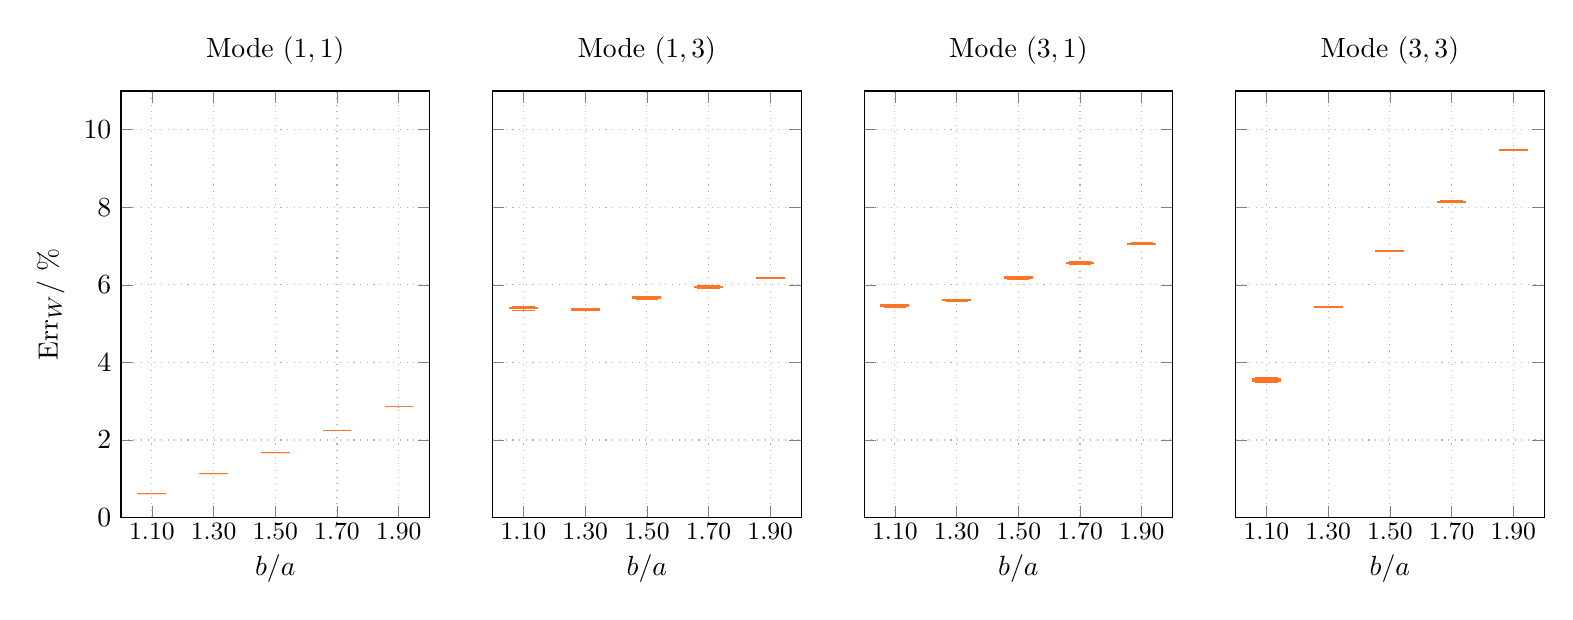
\begin{tikzpicture}
\begin{groupplot}[
    group style={
        group size=4 by 1,
        horizontal sep=0.8cm,
        vertical sep=0.4cm,
        y descriptions at=edge left,
        x descriptions at=edge bottom,
    },
    width=5.5cm, height=7cm,
    boxplot={
        draw direction=y,
        box extend=0.45,
    },
    xtick={1,2,3,4,5},
    xticklabels={1.10,1.30,1.50,1.70,1.90},
    xticklabel style={rotate=0, font=\small, inner sep=2pt},
    xmin=0.5, xmax=5.5,
    xlabel={$b/a$},
    ylabel={$\mathrm{Err}_W$/ \%},
    ymin=0, ymax=11,
    grid=both,
    grid style={dotted, gray!60},
]

\nextgroupplot[title={Mode $(1,1)$}]
\addplot [color=myorange, fill=myorange!20, boxplot/draw position=1, boxplot prepared={median=0.615, upper quartile=0.617, lower quartile=0.612, upper whisker=0.618, lower whisker=0.606}] coordinates {}; % b/a=1.10 own
% \addplot [color=mypurple, fill=mypurple!20, boxplot/draw position=1, boxplot prepared={median=1.609, upper quartile=1.620, lower quartile=1.597, upper whisker=1.628, lower whisker=1.580}] coordinates {}; % b/a=1.10 xl
\addplot [color=myorange, fill=myorange!20, boxplot/draw position=2, boxplot prepared={median=1.134, upper quartile=1.135, lower quartile=1.133, upper whisker=1.135, lower whisker=1.131}] coordinates {}; % b/a=1.30 own
% \addplot [color=mypurple, fill=mypurple!20, boxplot/draw position=2, boxplot prepared={median=1.733, upper quartile=1.740, lower quartile=1.725, upper whisker=1.744, lower whisker=1.716}] coordinates {}; % b/a=1.30 xl
\addplot [color=myorange, fill=myorange!20, boxplot/draw position=3, boxplot prepared={median=1.674, upper quartile=1.675, lower quartile=1.673, upper whisker=1.675, lower whisker=1.673}] coordinates {}; % b/a=1.50 own
% \addplot [color=mypurple, fill=mypurple!20, boxplot/draw position=3, boxplot prepared={median=1.921, upper quartile=1.928, lower quartile=1.912, upper whisker=1.933, lower whisker=1.899}] coordinates {}; % b/a=1.50 xl
\addplot [color=myorange, fill=myorange!20, boxplot/draw position=4, boxplot prepared={median=2.252, upper quartile=2.252, lower quartile=2.251, upper whisker=2.253, lower whisker=2.251}] coordinates {}; % b/a=1.70 own
% \addplot [color=mypurple, fill=mypurple!20, boxplot/draw position=4, boxplot prepared={median=2.088, upper quartile=2.094, lower quartile=2.081, upper whisker=2.097, lower whisker=2.069}] coordinates {}; % b/a=1.70 xl
\addplot [color=myorange, fill=myorange!20, boxplot/draw position=5, boxplot prepared={median=2.857, upper quartile=2.857, lower quartile=2.857, upper whisker=2.857, lower whisker=2.856}] coordinates {}; % b/a=1.90 own
% \addplot [color=mypurple, fill=mypurple!20, boxplot/draw position=5, boxplot prepared={median=2.214, upper quartile=2.218, lower quartile=2.208, upper whisker=2.220, lower whisker=2.202}] coordinates {}; % b/a=1.90 xl

\nextgroupplot[title={Mode $(1,3)$}]
\addplot [color=myorange, fill=myorange!20, boxplot/draw position=1, boxplot prepared={median=5.404, upper quartile=5.423, lower quartile=5.380, upper whisker=5.437, lower whisker=5.347}] coordinates {}; % b/a=1.10 own
% \addplot [color=mypurple, fill=mypurple!20, boxplot/draw position=1, boxplot prepared={median=2.463, upper quartile=2.488, lower quartile=2.442, upper whisker=2.509, lower whisker=2.422}] coordinates {}; % b/a=1.10 xl
\addplot [color=myorange, fill=myorange!20, boxplot/draw position=2, boxplot prepared={median=5.369, upper quartile=5.383, lower quartile=5.349, upper whisker=5.391, lower whisker=5.329}] coordinates {}; % b/a=1.30 own
% \addplot [color=mypurple, fill=mypurple!20, boxplot/draw position=2, boxplot prepared={median=1.464, upper quartile=1.479, lower quartile=1.445, upper whisker=1.488, lower whisker=1.428}] coordinates {}; % b/a=1.30 xl
\addplot [color=myorange, fill=myorange!20, boxplot/draw position=3, boxplot prepared={median=5.675, upper quartile=5.695, lower quartile=5.654, upper whisker=5.709, lower whisker=5.625}] coordinates {}; % b/a=1.50 own
% \addplot [color=mypurple, fill=mypurple!20, boxplot/draw position=3, boxplot prepared={median=1.414, upper quartile=1.435, lower quartile=1.391, upper whisker=1.451, lower whisker=1.362}] coordinates {}; % b/a=1.50 xl
\addplot [color=myorange, fill=myorange!20, boxplot/draw position=4, boxplot prepared={median=5.943, upper quartile=5.960, lower quartile=5.924, upper whisker=5.973, lower whisker=5.900}] coordinates {}; % b/a=1.70 own
% \addplot [color=mypurple, fill=mypurple!20, boxplot/draw position=4, boxplot prepared={median=1.492, upper quartile=1.510, lower quartile=1.472, upper whisker=1.524, lower whisker=1.447}] coordinates {}; % b/a=1.70 xl
\addplot [color=myorange, fill=myorange!20, boxplot/draw position=5, boxplot prepared={median=6.182, upper quartile=6.192, lower quartile=6.169, upper whisker=6.198, lower whisker=6.157}] coordinates {}; % b/a=1.90 own
% \addplot [color=mypurple, fill=mypurple!20, boxplot/draw position=5, boxplot prepared={median=1.612, upper quartile=1.622, lower quartile=1.599, upper whisker=1.628, lower whisker=1.586}] coordinates {}; % b/a=1.90 xl

\nextgroupplot[title={Mode $(3,1)$}]
\addplot [color=myorange, fill=myorange!20, boxplot/draw position=1, boxplot prepared={median=5.473, upper quartile=5.489, lower quartile=5.451, upper whisker=5.499, lower whisker=5.414}] coordinates {}; % b/a=1.10 own
% \addplot [color=mypurple, fill=mypurple!20, boxplot/draw position=1, boxplot prepared={median=1.533, upper quartile=1.553, lower quartile=1.515, upper whisker=1.570, lower whisker=1.502}] coordinates {}; % b/a=1.10 xl
\addplot [color=myorange, fill=myorange!20, boxplot/draw position=2, boxplot prepared={median=5.602, upper quartile=5.613, lower quartile=5.586, upper whisker=5.617, lower whisker=5.568}] coordinates {}; % b/a=1.30 own
% \addplot [color=mypurple, fill=mypurple!20, boxplot/draw position=2, boxplot prepared={median=0.916, upper quartile=0.926, lower quartile=0.898, upper whisker=0.931, lower whisker=0.878}] coordinates {}; % b/a=1.30 xl
\addplot [color=myorange, fill=myorange!20, boxplot/draw position=3, boxplot prepared={median=6.194, upper quartile=6.208, lower quartile=6.177, upper whisker=6.218, lower whisker=6.151}] coordinates {}; % b/a=1.50 own
% \addplot [color=mypurple, fill=mypurple!20, boxplot/draw position=3, boxplot prepared={median=1.078, upper quartile=1.091, lower quartile=1.064, upper whisker=1.102, lower whisker=1.048}] coordinates {}; % b/a=1.50 xl
\addplot [color=myorange, fill=myorange!20, boxplot/draw position=4, boxplot prepared={median=6.572, upper quartile=6.585, lower quartile=6.555, upper whisker=6.595, lower whisker=6.530}] coordinates {}; % b/a=1.70 own
% \addplot [color=mypurple, fill=mypurple!20, boxplot/draw position=4, boxplot prepared={median=1.799, upper quartile=1.821, lower quartile=1.780, upper whisker=1.839, lower whisker=1.758}] coordinates {}; % b/a=1.70 xl
\addplot [color=myorange, fill=myorange!20, boxplot/draw position=5, boxplot prepared={median=7.065, upper quartile=7.074, lower quartile=7.052, upper whisker=7.080, lower whisker=7.038}] coordinates {}; % b/a=1.90 own
% \addplot [color=mypurple, fill=mypurple!20, boxplot/draw position=5, boxplot prepared={median=0.975, upper quartile=0.981, lower quartile=0.964, upper whisker=0.983, lower whisker=0.949}] coordinates {}; % b/a=1.90 xl

\nextgroupplot[title={Mode $(3,3)$}]
\addplot [color=myorange, fill=myorange!20, boxplot/draw position=1, boxplot prepared={median=3.557, upper quartile=3.590, lower quartile=3.521, upper whisker=3.614, lower whisker=3.475}] coordinates {}; % b/a=1.10 own
% \addplot [color=mypurple, fill=mypurple!20, boxplot/draw position=1, boxplot prepared={median=1.293, upper quartile=1.356, lower quartile=1.232, upper whisker=1.406, lower whisker=1.168}] coordinates {}; % b/a=1.10 xl
\addplot [color=myorange, fill=myorange!20, boxplot/draw position=2, boxplot prepared={median=5.437, upper quartile=5.439, lower quartile=5.428, upper whisker=5.441, lower whisker=5.415}] coordinates {}; % b/a=1.30 own
% \addplot [color=mypurple, fill=mypurple!20, boxplot/draw position=2, boxplot prepared={median=3.039, upper quartile=3.042, lower quartile=3.032, upper whisker=3.048, lower whisker=3.017}] coordinates {}; % b/a=1.30 xl
\addplot [color=myorange, fill=myorange!20, boxplot/draw position=3, boxplot prepared={median=6.874, upper quartile=6.877, lower quartile=6.872, upper whisker=6.878, lower whisker=6.858}] coordinates {}; % b/a=1.50 own
% \addplot [color=mypurple, fill=mypurple!20, boxplot/draw position=3, boxplot prepared={median=1.969, upper quartile=1.974, lower quartile=1.961, upper whisker=1.977, lower whisker=1.933}] coordinates {}; % b/a=1.50 xl
\addplot [color=myorange, fill=myorange!20, boxplot/draw position=4, boxplot prepared={median=8.146, upper quartile=8.159, lower quartile=8.132, upper whisker=8.170, lower whisker=8.115}] coordinates {}; % b/a=1.70 own
% \addplot [color=mypurple, fill=mypurple!20, boxplot/draw position=4, boxplot prepared={median=1.499, upper quartile=1.512, lower quartile=1.476, upper whisker=1.519, lower whisker=1.434}] coordinates {}; % b/a=1.70 xl
\addplot [color=myorange, fill=myorange!20, boxplot/draw position=5, boxplot prepared={median=9.480, upper quartile=9.489, lower quartile=9.469, upper whisker=9.495, lower whisker=9.460}] coordinates {}; % b/a=1.90 own
% \addplot [color=mypurple, fill=mypurple!20, boxplot/draw position=5, boxplot prepared={median=1.642, upper quartile=1.652, lower quartile=1.626, upper whisker=1.657, lower whisker=1.607}] coordinates {}; % b/a=1.90 xl

\end{groupplot}
\end{tikzpicture}
\end{document}
